\chapter{Radicales, carbenos y transposiciones}\label{ch:b3:radicals-carbenes}

El pelitre se defiende con ésteres del ácido crisantémico, moléculas
construidas en torno a un anillo de tres carbonos; sus parientes sintéticos figuran entre
los insecticidas domésticos más usados. Los químicos cierran esos anillos en una sola etapa
adicionando un \omterm{def:b3:organometallic-bonding:carbene}{carbeno} a un doble enlace: un átomo de carbono con solo seis electrones
a su alrededor, dos de ellos no compartidos. Este capítulo trata de los intermedios reactivos
que los volúmenes del primer y del segundo año solo encontraron de pasada (los radicales usados en
síntesis, los \omterm{def:b3:organometallic-bonding:carbene}{carbenos} y los \omterm{def:b3:radicals-carbenes:nitrene}{nitrenos}) y de las transposiciones en las que un grupo
se desplaza hacia un átomo de carbono, nitrógeno u oxígeno deficiente en electrones, entre ellas dos
que fabrican los monómeros del nailon 6 y de un poliéster biodegradable a partir de la
misma cetona.

\begin{recall}
El volumen del primer año introdujo los radicales, la homólisis y las flechas de media punta,
los carbocationes y sus transposiciones, los nucleófilos y los grupos salientes; el
volumen del segundo año, las reacciones radicalarias en cadena (iniciación, propagación, terminación, iniciadores
radicalarios), los peroxiácidos, las lactonas, las lactamas y las iminas.
El \cref{ch:b3:complex-kinetics} trató la cinética de las \omterm{def:b3:complex-kinetics:chain}{reacciones en cadena};
el \cref{ch:b3:organometallic-bonding}, los \omterm{def:b3:organometallic-bonding:carbene}{carbenos} como ligandos;
el \cref{ch:b3:many-electron-atoms}, los \omterm{def:b3:many-electron-atoms:singlet-triplet}{estados singlete} y triplete, y
el \cref{ch:b3:rate-theories}, el postulado de Hammond.
\end{recall}

\begin{omfigure}
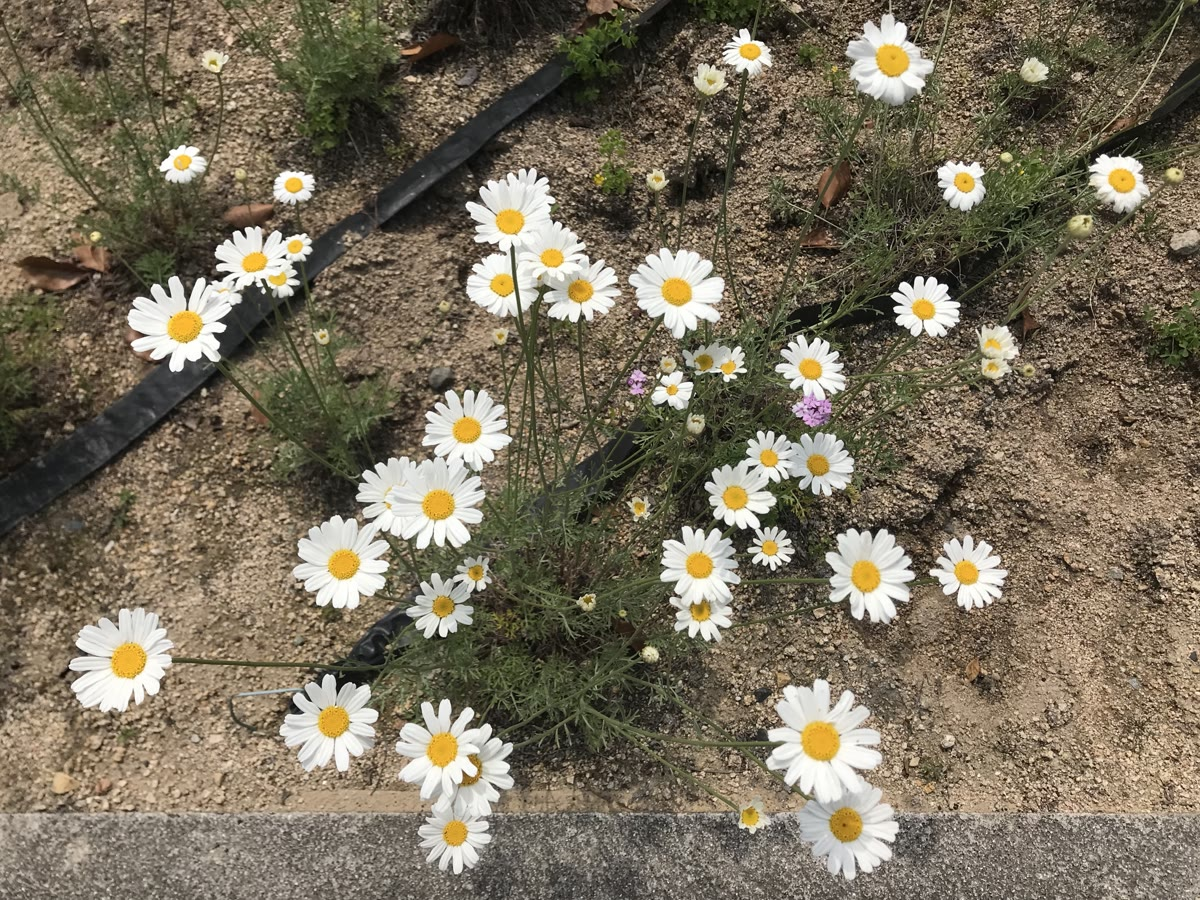
\includegraphics[width=0.48\linewidth]{images/book4/pyrethrum.jpg}

{\small Flores de pelitre. Contienen las piretrinas, ésteres insecticidas
de un ácido ciclopropanocarboxílico. Fotografía: Soramimi, CC BY-SA 4.0.}
\end{omfigure}

\section{Reacciones radicalarias en cadena en síntesis}

La estabilidad de un radical carbonado se mide por la entalpía de disociación
del enlace C--H que lo formaría: cuanto más débil es el enlace, más
estable es el radical.

\begin{proposition}[Entalpías de disociación de enlace]\label{prop:b3:radicals-carbenes:bde}
La entalpía de disociación del enlace R--H a \qty{298}{K} se deduce de las entalpías de formación en fase gaseosa:
$\mathrm{BDE(R{-}H)} = \Delta_fH^\circ(\mathrm R^\bullet) + \Delta_fH^\circ(\mathrm H^\bullet) - \Delta_fH^\circ(\mathrm{RH})$.
\end{proposition}

\begin{proof}
La homólisis $\mathrm{RH \to R^\bullet + H^\bullet}$ tiene, por la ley de Hess, como entalpía de reacción la de formación de los productos
menos la del reactivo; esa entalpía de reacción es, por definición, la entalpía de disociación
del enlace.
\end{proof}

\begin{omfigure}
% ledger: dfh4:CH3r, dfh4:C2H5r, dfh4:iC3H7r, dfh4:tC4H9r, dfh4:PhCH2r, dfh4:H, dfh:CH4_g, dfh:C2H6_g, dfh:C3H8_g, dfh4:iC4H10, dfh4:toluene_g
\begin{tikzpicture}
\begin{axis}[width=0.72\linewidth, height=5.2cm, ybar, bar width=16pt, ymin=350, ymax=450,
  xtick={1,2,3,4,5}, xticklabels={{$\ce{CH3-H}$}, {$\ce{C2H5-H}$}, {$\mathrm{(CH_3)_2CH{-}H}$}, {$\mathrm{(CH_3)_3C{-}H}$}, {$\ce{C6H5CH2-H}$}},
  x tick label style={font=\scriptsize}, ylabel={BDE / \unit{kJ.mol^{-1}}},
  axis lines=left, tick label style={font=\scriptsize}, label style={font=\small},
  nodes near coords, nodes near coords style={font=\scriptsize, /pgf/number format/fixed, /pgf/number format/precision=0},
  enlarge x limits=0.15]
\addplot[fill=omDef!55, draw=omDef] table[x=i, y=bde] {figdata/out/bachelor-3-bde.dat};
\end{axis}
\end{tikzpicture}

{\small Entalpías de disociación de enlaces C--H a \qty{298}{K}, calculadas a partir de las entalpías de
formación en fase gaseosa de las moléculas y de los radicales: metilo, primario,
secundario, terciario y bencílico. El enlace se debilita a medida que el radical formado está
más sustituido o conjugado.}
\end{omfigure}

\begin{proposition}[Selectividad de la halogenación]\label{prop:b3:radicals-carbenes:halogenation-selectivity}
La abstracción de hidrógeno por un átomo de bromo es mucho más selectiva entre los enlaces C--H primarios,
secundarios y terciarios que la abstracción por un átomo de cloro.
\end{proposition}

\begin{proof}[Argumento]
Como $\mathrm{BDE(H{-}Cl)}$ es mayor que todos los valores C--H de la figura y $\mathrm{BDE(H{-}Br)}$ menor,
la abstracción por el cloro es exotérmica, y por el bromo, endotérmica. Según el postulado
de Hammond (\cref{ch:b3:rate-theories}), el estado de transición del cloro es temprano,
parecido a los reactivos, y apenas percibe la diferencia entre los radicales formados;
el del bromo es tardío, parecido a los productos, y su energía de activación sigue la mayor parte de
la diferencia de BDE, que el factor de Boltzmann convierte en grandes cocientes de velocidad.
\end{proof}

El hidruro de tributilestaño reduce los haluros de alquilo mediante una cadena: un radical estaño toma el
halógeno, el radical alquilo toma un átomo de hidrógeno de la siguiente molécula de
hidruro, y se forma un nuevo radical estaño. La misma cadena elimina un grupo hidroxi
una vez convertido en un tiocarbonil éster (la desoxigenación de
Barton--McCombie) y cierra anillos. Los residuos de organoestaño son tóxicos y difíciles de
eliminar; el tris(trimetilsilil)silano y otros silanos sustituyen hoy a menudo al hidruro
de estaño.

\begin{omfigure}
\begin{tikzpicture}[font=\small, >=Stealth]
  \node (a) at (-2.0,0) {$\mathrm{Bu_3Sn^\bullet}$};
  \node (b) at (2.0,0) {$\mathrm{R^\bullet}$};
  \draw[->, thick] (a) to[bend left=35] node[midway, above, font=\scriptsize] {$+\,$R--Br, $\ -\,\mathrm{Bu_3SnBr}$} (b);
  \draw[->, thick] (b) to[bend left=35] node[midway, below, font=\scriptsize] {$+\,\mathrm{Bu_3SnH}$, $\ -\,$R--H} (a);
  \node[font=\scriptsize, align=center, anchor=north] at (0,-1.5) {iniciación: AIBN $\xrightarrow{\Delta}$ 2 R$'^\bullet$ $+$ $\ce{N2}$; \ R$'^\bullet$ $+$ $\mathrm{Bu_3SnH}$ $\to$ R$'$H $+$ $\mathrm{Bu_3Sn^\bullet}$};
\end{tikzpicture}

{\small Las etapas de propagación de una reducción de un bromuro de alquilo con hidruro de estaño.
Cada R--Br reducido consume un $\mathrm{Bu_3SnH}$ y da un $\mathrm{Bu_3SnBr}$; los \omterm{def:b3:complex-kinetics:chain}{portadores de cadena}
son el radical estaño y el radical alquilo.}
\end{omfigure}

El bromuro de hidrógeno se adiciona a los alquenos mediante el mismo tipo de cadena cuando hay
peróxidos: un átomo de bromo se adiciona al extremo menos sustituido, lo que da el radical más
estable, que toma después un átomo de hidrógeno del HBr: adición
anti-Markovnikov.

\section{Ciclaciones radicalarias}

\begin{definition}[Ciclaciones exo y endo]\label{def:b3:radicals-carbenes:cyclisation}
En una \emph{ciclación exo}\index{ciclacion exo@ciclación exo}, el enlace que se rompe (o
el enlace $\pi$ atacado) queda fuera del nuevo anillo; en una \emph{ciclación
endo}\index{ciclacion endo@ciclación endo}, dentro de él.
\end{definition}

\begin{omfigure}
\begin{tikzpicture}[font=\scriptsize, >=Stealth]
  % hex-5-enyl radical: C1 radical, C5=C6
  \foreach \i/\a in {1/162, 2/234, 3/306, 4/18} { \coordinate (p\i) at (\a:0.9); }
  \coordinate (p5) at (90:0.95); \coordinate (p6) at (90:1.9);
  \draw[thick] (p1) -- (p2) -- (p3) -- (p4) -- (p5);
  \draw[thick, double, double distance=1.5pt] (p5) -- (p6);
  \node[anchor=east] at (p1) {$\bullet$\,1};
  \node[anchor=west] at (p5) {5}; \node[anchor=west] at (p6) {6};
  \draw[->, omMeth, thick] ($(p1)+(0.1,0.15)$) to[bend left=25] node[pos=0.45, below right, inner sep=1pt] {5-exo} ($(p5)+(-0.15,-0.05)$);
  \draw[->, omThm, thick, densely dashed] ($(p1)+(0,0.25)$) to[bend left=50] node[midway, left] {6-endo} ($(p6)+(-0.2,0)$);
  \node[font=\small, align=center] at (0,-1.6) {radical hex-5-enilo};
  \draw[->, thick] (1.6,0.3) -- (2.7,0.3) node[midway, above] {rápida};
  \begin{scope}[xshift=4.0cm]
    \foreach \i/\a in {1/162, 2/234, 3/306, 4/18, 5/90} { \coordinate (q\i) at (\a:0.75); }
    \draw[thick] (q1) -- (q2) -- (q3) -- (q4) -- (q5) -- (q1);
    \draw[thick] (q5) -- ++(90:0.6) coordinate (q6);
    \node[anchor=south, inner sep=1pt] at (q6) {$\mathrm{{}^\bullet CH_2}$};
    \node[font=\small, align=center] at (0,-1.6) {radical ciclopentilmetilo};
  \end{scope}
\end{tikzpicture}

{\small El radical 5-hexenilo se cierra por ataque de C1 sobre C5 (5-exo, verde): el
nuevo anillo tiene cinco miembros y el radical queda fuera de él, en C6. El ataque sobre C6
(6-endo, trazo discontinuo rojo) daría el radical ciclohexilo secundario, más estable,
pero es mucho más lento: la cadena no puede situar C1 en la línea de aproximación a C6 que
exige el orbital $\pi^*$.}
\end{omfigure}

\begin{proposition}[Reglas de Baldwin]\label{prop:b3:radicals-carbenes:baldwin}
Para los cierres de anillo (establecidas experimentalmente, con una justificación
estereoelectrónica): sobre un carbono tetraédrico (tet), los cierres 3- a 7-exo están favorecidos, y los 5- y
6-endo, desfavorecidos; sobre un carbono trigonal (trig), los 3- a 7-exo están favorecidos, los 3- a 5-endo,
desfavorecidos, y los 6- y 7-endo, favorecidos; sobre un carbono digonal (dig), los 3- y 4-exo están
desfavorecidos, los 5- a 7-exo, favorecidos, y los 3- a 7-endo, favorecidos.
\end{proposition}

La justificación es el ángulo de ataque que necesita cada tipo de enlace: por detrás del
enlace en un carbono tet, a unos 107° respecto de un sistema $\pi$ trigonal, y a un ángulo más
estrecho respecto de un triple enlace; una cadena corta no puede alcanzar esas posiciones en los
casos desfavorecidos.

\begin{definition}[Reloj radicalario]\label{def:b3:radicals-carbenes:radical-clock}
Un \emph{reloj radicalario}\index{reloj radicalario} es un radical que se transpone
de forma unimolecular con una constante de velocidad conocida, como el radical 5-hexenilo
al ciclarse; su competencia con una trampa bimolecular mide la constante de velocidad
de la trampa, o a la inversa.
\end{definition}

\begin{proposition}[Cinética de competencia]\label{prop:b3:radicals-carbenes:clock}
Si un radical se cicla ($k_c$) o es atrapado por un hidruro mantenido en exceso a la
concentración $[\mathrm{R_3SnH}]$ ($k_H$), la razón de productos es
$[\text{ciclado}]/[\text{directo}] = k_c/(k_H[\mathrm{R_3SnH}])$.
\end{proposition}

\begin{proof}
En cada instante, el producto ciclado y el producto directo se forman a las velocidades $k_c[\mathrm R^\bullet]$ y $k_H[\mathrm{R_3SnH}][\mathrm R^\bullet]$. Su cociente
no depende de la concentración de radical, que varía; con la concentración de hidruro
constante, la integración en el tiempo multiplica ambas por la misma
$\int[\mathrm R^\bullet]\,\dd t$, y la razón de los productos es el cociente de las constantes de velocidad
multiplicado por $1/[\mathrm{R_3SnH}]$.
\end{proof}

\begin{omfigure}
\begin{tikzpicture}
\begin{axis}[name=a, width=0.47\linewidth, height=5.2cm, xmode=log, xmin=1e-3, xmax=1, ymin=0, ymax=1,
  axis lines=left, xlabel={$[\mathrm{Bu_3SnH}]$ / \unit{mol.L^{-1}}}, ylabel={fracción ciclada},
  tick label style={font=\scriptsize}, label style={font=\small}]
\addplot[omDef, thick] table[x=c, y=fcyc] {figdata/out/bachelor-3-radical-clock.dat};
\end{axis}
\begin{axis}[at={(a.east)}, anchor=west, xshift=1.5cm, width=0.47\linewidth, height=5.2cm,
  xmin=0, xmax=1, ymin=0, ymax=11, axis lines=left,
  xlabel={$[\mathrm{Bu_3SnH}]$ / \unit{mol.L^{-1}}}, ylabel={[directo]/[ciclado]},
  tick label style={font=\scriptsize}, label style={font=\small}]
\addplot[omThm, thick] table[x=c, y=inv] {figdata/out/bachelor-3-radical-clock-b.dat};
\node[font=\scriptsize, anchor=west, omThm] at (axis cs:0.15,7.5) {pendiente $k_H/k_c$};
\end{axis}
\end{tikzpicture}

{\small El reloj del 5-hexenilo con las constantes de velocidad del modelo $k_c = \qty{2.3e5}{s^{-1}}$ y
$k_H = \qty{2.4e6}{L.mol^{-1}.s^{-1}}$. Izquierda: fracción de metilciclopentano entre los productos en función de la
concentración de hidruro: la mitad en $k_c/k_H \approx \qty{0.1}{mol/L}$. Derecha: la razón inversa es una recta
que pasa por el origen, de pendiente $k_H/k_c$.}
\end{omfigure}

\begin{method}[Diseñar una reducción o una ciclación radicalaria]\label{met:b3:radicals-carbenes:radical-chain}
\begin{enumerate}
  \item Para una reducción simple, mantener concentrado el dador de hidrógeno (unos
        \qty{0.1}{mol/L} o más) para que el radical sea atrapado antes de transponerse.
  \item Para una ciclación, mantener diluido el dador, o añadirlo lentamente, para que el
        radical se cicle primero: elegir $[\text{dador}] \ll k_c/k_H$.
  \item Elegir un iniciador cuyo tiempo de semirreacción a la temperatura de reacción sea del
        orden del tiempo de reacción (AIBN hacia \qty{80}{\celsius}), y añadirlo en porciones si
        es necesario.
  \item Preferir un silano u otro dador sin estaño, y eliminar el oxígeno, que atrapa
        los radicales carbonados.
\end{enumerate}
\end{method}

\begin{inthelab}[Adición lenta con una bomba de jeringa]
Para mantener diluido un reactivo durante toda una reacción, su disolución se carga en una
jeringa estanca a los gases y se añade a través de un septo con una bomba de jeringa durante varias
horas, sobre la disolución del sustrato a reflujo bajo nitrógeno. La
concentración del reactivo se mantiene entonces cerca de su bajo valor estacionario, fijado por
la velocidad de adición y la velocidad a la que se consume.
\end{inthelab}

\section{Carbenos}

\begin{definition}[Carbenos singlete y triplete]\label{def:b3:radicals-carbenes:carbene-states}
Un \emph{carbeno singlete}\index{carbeno singlete} tiene sus dos electrones no
enlazantes apareados en un mismo orbital, un híbrido $sp^2$, y su orbital p vacío; un
\emph{carbeno triplete}\index{carbeno triplete} los tiene desapareados, uno en cada
orbital, con espines paralelos.
\end{definition}

\begin{omfigure}
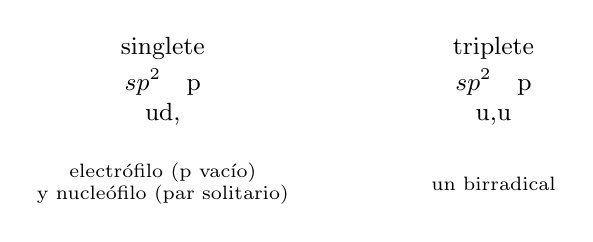
\begin{tikzpicture}[font=\small]
  \node[align=center] at (0,0) {singlete\\[2pt] $sp^2$ \ \ p\\ \omorbs{ud,}};
  \node[align=center] at (4.2,0) {triplete\\[2pt] $sp^2$ \ \ p\\ \omorbs{u,u}};
  \node[font=\scriptsize, align=center] at (0,-1.3) {electrófilo (p vacío)\\ y nucleófilo (par solitario)};
  \node[font=\scriptsize, align=center] at (4.2,-1.3) {un birradical};
\end{tikzpicture}

{\small Ocupación electrónica de los dos orbitales no enlazantes de un \omterm{def:b3:organometallic-bonding:carbene}{carbeno}. El
triplete es el estado fundamental del $\ce{CH2}$; los sustituyentes $\pi$-dadores (Cl, OR, $\mathrm{NR_2}$) elevan el
orbital p y hacen del singlete el estado fundamental, como en el diclorocarbeno.}
\end{omfigure}

Los \omterm{def:b3:organometallic-bonding:carbene}{carbenos} se obtienen por pérdida de dinitrógeno de un compuesto diazo (por calor, por luz
o con un catalizador metálico), por $\alpha$-eliminación (el cloroformo y una base fuerte dan
$\ce{CCl3-}$, que pierde un cloruro y da $\ce{CCl2}$), o bien se evitan por completo mediante un
\omterm{def:b3:radicals-carbenes:carbenoid}{carbenoide}.

\begin{definition}[Carbenoides]\label{def:b3:radicals-carbenes:carbenoid}
Un \emph{carbenoide}\index{carbenoide} es una especie unida a un metal que transfiere un
grupo \omterm{def:b3:organometallic-bonding:carbene}{carbeno} como lo haría un \omterm{def:b3:organometallic-bonding:carbene}{carbeno} libre, sin que llegue a formarse el \omterm{def:b3:organometallic-bonding:carbene}{carbeno} libre,
como el yoduro de yodometilcinc $\ce{ICH2ZnI}$ de la reacción de Simmons--Smith.
\end{definition}

\begin{definition}[Ciclopropanación]\label{def:b3:radicals-carbenes:cyclopropanation}
La \emph{ciclopropanación}\index{ciclopropanacion@ciclopropanación} es la formación de un
ciclopropano por adición de un \omterm{def:b3:organometallic-bonding:carbene}{carbeno} o de un \omterm{def:b3:radicals-carbenes:carbenoid}{carbenoide} a un doble enlace C=C.
\end{definition}

\begin{proposition}[La prueba de Skell]\label{prop:b3:radicals-carbenes:skell}
Un \omterm{def:b3:radicals-carbenes:carbene-states}{carbeno singlete} se adiciona a un alqueno \textit{cis} o \textit{trans} de forma estereoespecífica, conservando la
configuración relativa; un \omterm{def:b3:radicals-carbenes:carbene-states}{carbeno triplete} da los dos estereoisómeros del
ciclopropano.
\end{proposition}

\begin{proof}[Argumento]
El singlete forma los dos nuevos enlaces en una sola etapa concertada, sin tiempo para
la rotación. El triplete forma primero un enlace, lo que da un 1,3-birradical triplete; sus
dos electrones desapareados no pueden formar el segundo enlace hasta que se invierte un espín, lo que es
lento comparado con la rotación en torno al enlace sencillo C--C restante: la
configuración se pierde.
\end{proof}

\begin{omfigure}
\setchemfig{atom sep=1.8em}
\schemestart
\chemfig{H_3C-[:30]=[:0]-[:-30]CH_3}
\arrow{->[$\ce{CH2}$ singlete]}[,1.6]
\chemfig{(<[:210]H_3C)-[:0](<[:330]CH_3)-[:120]-[:240]}
\schemestop
\par\medskip

{\small La prueba de Skell: el \textit{cis}-but-2-eno, con los dos grupos metilo del mismo lado, da con
un \omterm{def:b3:radicals-carbenes:carbene-states}{carbeno singlete} solo \textit{cis}-1,2-dimetilciclopropano (los dos grupos metilo en cuñas,
en la misma cara del anillo); con un \omterm{def:b3:radicals-carbenes:carbene-states}{carbeno
triplete} aparece también el isómero \textit{trans}.}
\end{omfigure}

Los \omterm{def:b3:radicals-carbenes:carbene-states}{carbenos singlete} se insertan también en los enlaces C--H. Los carboxilatos de rodio(II)
descomponen los diazoésteres en \omterm{def:b3:radicals-carbenes:carbenoid}{carbenoides} de rodio que ciclopropanan los alquenos y se
insertan en los enlaces C--H de forma selectiva y, con ligandos quirales, enantioselectiva.

\begin{definition}[Nitrenos]\label{def:b3:radicals-carbenes:nitrene}
Un \emph{nitreno}\index{nitreno} $\mathrm{R{-}\ddot N}$ es el análogo nitrogenado de un \omterm{def:b3:organometallic-bonding:carbene}{carbeno}, un átomo de
nitrógeno neutro con solo seis electrones, formado por ejemplo por pérdida de
dinitrógeno de una azida.
\end{definition}

\section{Transposiciones hacia un carbono deficiente en electrones}

\begin{definition}[Desplazamiento 1,2]\label{def:b3:radicals-carbenes:shift}
Un \emph{desplazamiento 1,2}\index{desplazamiento 1,2} es el paso de un grupo, con su par
enlazante, de un átomo al átomo vecino deficiente en electrones.
\end{definition}

En un desplazamiento de Wagner--Meerwein, un grupo alquilo o un hidruro pasa a un carbocatión
vecino, lo que da uno más estable: las transposiciones de carbocationes del
volumen del primer año, ahora con su mecanismo nombrado. En la naturaleza, los esqueletos terpénicos se remodelan
mediante cascadas de tales desplazamientos.

\begin{definition}[Transposición pinacolínica]\label{def:b3:radicals-carbenes:pinacol}
La \emph{transposición pinacolínica}\index{transposicion pinacolinica@transposición pinacolínica} convierte un 1,2-diol,
en medio ácido, en una cetona o un aldehído: un grupo hidroxi sale en forma de agua, un
grupo del carbono vecino se desplaza hacia el catión, y el catión formado,
estabilizado por el oxígeno restante, pierde un protón.
\end{definition}

\begin{definition}[Aptitud migratoria]\label{def:b3:radicals-carbenes:migratory}
La \emph{aptitud migratoria}\index{aptitud migratoria} de un grupo es su
tendencia relativa a desplazarse, en un \omterm{def:b3:radicals-carbenes:shift}{desplazamiento 1,2}, hacia un centro deficiente en electrones.
\end{definition}

Los grupos que soportan bien la carga positiva durante el desplazamiento son los que mejor migran: el hidruro,
el arilo y el alquilo terciario antes que el secundario, el primario y el metilo. El pinacol,
$\mathrm{(CH_3)_2C(OH){-}C(OH)(CH_3)_2}$, da la pinacolona, 3,3-dimetilbutan-2-ona.

\begin{method}[Predecir el producto de una transposición]\label{met:b3:radicals-carbenes:rearrangement}
\begin{enumerate}
  \item Encontrar el átomo deficiente en electrones que se forma (catión, nitrenio, oxígeno de un
        peróxido activado, \omterm{def:b3:organometallic-bonding:carbene}{carbeno} o \omterm{def:b3:radicals-carbenes:nitrene}{nitreno}) y el grupo saliente que lo genera.
  \item Enumerar los grupos del átomo vecino que podrían desplazarse; cuando la
        geometría está fijada (oximas), solo puede hacerlo el grupo anti respecto del grupo saliente.
  \item En los demás casos, elegir según la \omterm{def:b3:radicals-carbenes:migratory}{aptitud migratoria}, o según qué grupo forma el catión más
        estable allí de donde sale.
  \item Desplazar el grupo con retención de su configuración y completar después el
        mecanismo (pérdida de un protón, adición de agua).
\end{enumerate}
\end{method}

\section{Transposiciones hacia un nitrógeno o un oxígeno deficientes en electrones}

\begin{definition}[Transposición de Beckmann]\label{def:b3:radicals-carbenes:beckmann}
La \emph{transposición de Beckmann}\index{transposicion de Beckmann@transposición de Beckmann} convierte una oxima,
en ácido fuerte, en una amida: el grupo hidroxi, activado como grupo saliente,
se va mientras el grupo situado en anti respecto de él se desplaza del carbono al nitrógeno; el agua se adiciona
al ion nitrilio formado, y la tautomerización da la amida.
\end{definition}

\begin{proposition}[Desplazamiento anti]\label{prop:b3:radicals-carbenes:beckmann-anti}
En la \omterm{def:b3:radicals-carbenes:beckmann}{transposición de Beckmann}, el grupo que se desplaza es el situado en anti respecto del
grupo saliente del nitrógeno.
\end{proposition}

\begin{proof}[Argumento]
El par enlazante que se desplaza ataca al nitrógeno por detrás del enlace N--O, como en una
sustitución $\mathrm S_\mathrm N2$; solo el grupo anti respecto del oxígeno tiene su enlace alineado con
el orbital $\sigma^*$ N--O. La etapa es concertada con la salida del grupo saliente,
de modo que no se forma ningún ion nitrenio libre que pudiera elegir de otro modo.
\end{proof}

\begin{omfigure}
\setchemfig{atom sep=1.9em}
\schemestart
\chemfig{*6(-----(=N-[:30]OH)-)}
\arrow{->[$\ce{H2SO4}$ (óleum)][Beckmann]}[,1.8]
\chemfig{*7(---N(-[:-90]H)-(=O)---)}
\schemestop
\par\medskip
\schemestart
\chemfig{*6(-----(=O)-)}
\arrow{->[peroxiácido][Baeyer--Villiger]}[,1.8]
\chemfig{*7(-----O-(=O)-)}
\schemestop

{\small Dos expansiones de anillo de la ciclohexanona. Arriba: su oxima se transpone en
óleum a caprolactama (azepan-2-ona), el monómero del nailon 6, con entrada del nitrógeno en
el anillo. Abajo: un peroxiácido inserta un átomo de oxígeno junto al grupo
carbonilo, lo que da la $\varepsilon$-caprolactona (oxepan-2-ona).}
\end{omfigure}

\begin{definition}[Oxidación de Baeyer--Villiger]\label{def:b3:radicals-carbenes:baeyer}
La \emph{oxidación de Baeyer--Villiger}\index{oxidacion de Baeyer--Villiger@oxidación de Baeyer--Villiger} convierte una
cetona en un éster, o una cetona cíclica en una lactona, con un peroxiácido: el
peroxiácido se adiciona al grupo carbonilo, y después un grupo del carbono carbonílico
se desplaza hacia el oxígeno peroxídico más cercano mientras sale un carboxilato.
\end{definition}

\begin{proposition}[Regioquímica de Baeyer--Villiger]\label{prop:b3:radicals-carbenes:bv-retention}
En la \omterm{def:b3:radicals-carbenes:baeyer}{oxidación de Baeyer--Villiger}, el grupo que se desplaza conserva su
configuración, y el orden de \omterm{def:b3:radicals-carbenes:migratory}{aptitud migratoria} es alquilo terciario >
alquilo secundario $\approx$ arilo > alquilo primario > metilo (establecido experimentalmente).
\end{proposition}

\begin{proof}[Argumento]
El grupo se desplaza con su par enlazante a través de la cara del carbono que abandona
y llega al oxígeno por el mismo lado, de modo que su configuración se conserva. En el
estado de transición, el grupo que se desplaza soporta una carga positiva parcial, que
estabilizan la sustitución alquílica y la conjugación arílica.
\end{proof}

\begin{definition}[Isocianatos, transposiciones de Curtius y de Hofmann]\label{def:b3:radicals-carbenes:curtius}
Un \emph{isocianato}\index{isocianato} es un compuesto $\ce{R-N=C=O}$. En la \emph{transposición de Curtius}%
\index{transposicion de Curtius@transposición de Curtius}, una azida de acilo pierde dinitrógeno al
calentarla mientras el grupo R pasa del carbono al nitrógeno, lo que da un isocianato;
en la \emph{transposición de Hofmann}\index{transposicion de Hofmann@transposición de Hofmann}, una amida primaria
tratada con bromo y una base da el mismo isocianato a través de una
N-bromoamida. Con agua, el isocianato da la amina $\ce{RNH2}$ y dióxido de
carbono; con un alcohol, un carbamato.
\end{definition}

\begin{definition}[Cetenos y transposición de Wolff]\label{def:b3:radicals-carbenes:wolff}
Un \emph{ceteno}\index{ceteno} es un compuesto $\mathrm{R_2C{=}C{=}O}$. En la \emph{transposición de Wolff}%
\index{transposicion de Wolff@transposición de Wolff}, una $\alpha$-diazocetona pierde dinitrógeno
mientras el grupo del carbono carbonílico se desplaza, lo que da un ceteno, que adiciona
agua, un alcohol o una amina.
\end{definition}

La \omterm{def:b3:radicals-carbenes:wolff}{transposición de Wolff} es la etapa clave de la homologación de Arndt--Eistert,
que alarga un ácido carboxílico en un carbono: cloruro de ácido, después
diazocetona, después \omterm{def:b3:radicals-carbenes:wolff}{ceteno}, después el ácido homólogo.

\begin{safety}{\ghs[0.62cm]{GHS06}\ghs[0.62cm]{GHS08}\ghs[0.62cm]{GHS09}}
% ledger: ghs4:Bu3SnH, ghs4:diazomethane, ghs4:AIBN
Hidruro de tributilestaño: tóxico en caso de ingestión, nocivo en contacto con la piel, perjudica a determinados órganos
por exposición prolongada, muy tóxico para los organismos acuáticos; los residuos de estaño se recogen
por separado. El diazometano es un gas tóxico, cancerígeno y explosivo; se
nombra aquí solo por su química y en la práctica se sustituye por reactivos más seguros,
como el trimetilsilildiazometano. El AIBN es autorreactivo al calentarlo.
\end{safety}

\begin{history}[Un radical que no debería existir, y un nailon]
En 1900, Moses Gomberg, al intentar preparar hexafeniletano, obtuvo una disolución
amarilla que absorbía oxígeno y yodo: el radical trifenilmetilo, el primer
radical carbonado persistente. Medio siglo después, la \omterm{def:b3:radicals-carbenes:beckmann}{transposición de Beckmann} de la
oxima de la ciclohexanona se convirtió en la ruta industrial hacia la caprolactama, polimerizada por
apertura de anillo en nailon 6, una fibra y un plástico técnico fabricados a muy gran
escala.
\end{history}

\section{Ejercicios}

\begin{exercise}[$\star$]\label{exo:b3:radicals-carbenes:1}
A \qty{25}{\celsius}, las reactividades relativas por hidrógeno de los enlaces C--H primarios, secundarios y
terciarios son $1 : 3.9 : 5.1$ frente a los átomos de cloro y $1 : 82 : 1600$ frente a los
átomos de bromo (datos del ejercicio). Calcúlense las proporciones de 1- y 2-halopropano
formadas a partir del propano en cada caso.
\end{exercise}

\begin{exercise}[$\star$]\label{exo:b3:radicals-carbenes:2}
¿Cuál es el estado fundamental del $\ce{CH2}$, y el del $\ce{CCl2}$? ¿Cuál se adiciona de forma estereoespecífica al
\textit{trans}-but-2-eno, y qué da?
\end{exercise}

\begin{exercise}[$\star$]\label{exo:b3:radicals-carbenes:3}
Dese el producto de la reacción de Simmons--Smith del (\textit{Z})-hex-3-eno.
\end{exercise}

\begin{exercise}[$\star$]\label{exo:b3:radicals-carbenes:4}
Dense los productos de la \omterm{def:b3:radicals-carbenes:baeyer}{oxidación de Baeyer--Villiger} de la ciclohexanona y de la
acetofenona.
\end{exercise}

\begin{exercise}[$\star\star$]\label{exo:b3:radicals-carbenes:5}
Con los datos del \cref{exo:b3:radicals-carbenes:1}, calcúlense las proporciones de
los dos monocloruros y de los dos monobromuros del 2-metilpropano.
\end{exercise}

\begin{exercise}[$\star\star$]\label{exo:b3:radicals-carbenes:6}
Un nuevo \omterm{def:b3:radicals-carbenes:radical-clock}{reloj radicalario}, reducido con $\qty{0.020}{mol/L}$ de $\mathrm{Bu_3SnH}$, da tres veces más producto transpuesto
que no transpuesto. Con $k_H = \qty{2.4e6}{L.mol^{-1}.s^{-1}}$, encuéntrese su constante de velocidad.
\end{exercise}

\begin{exercise}[$\star\star$]\label{exo:b3:radicals-carbenes:7}
Clasifíquese según las reglas de Baldwin el ataque de un radical hex-5-enilo sobre C5 y sobre C6,
y dígase después si cada uno de estos cierres está favorecido: 4-exo-tet, 5-endo-trig,
5-exo-dig, 3-exo-dig, 5-endo-dig.
\end{exercise}

\begin{exercise}[$\star\star$]\label{exo:b3:radicals-carbenes:8}
Dese el producto de la \omterm{def:b3:radicals-carbenes:pinacol}{transposición pinacolínica} del 2,3-difenilbutano-2,3-diol,
y explíquese la elección del grupo que se desplaza.
\end{exercise}

\begin{exercise}[$\star\star$]\label{exo:b3:radicals-carbenes:9}
Se calienta azida de benzoílo en tolueno y después se añade agua; en un segundo experimento,
etanol. Dense los productos.
\end{exercise}

\begin{exercise}[$\star\star\star$]\label{exo:b3:radicals-carbenes:10}
Con $\mathrm{BDE(H{-}Cl)} = \qty{432}{kJ/mol}$ y $\mathrm{BDE(H{-}Br)} = \qty{366}{kJ/mol}$ (datos del ejercicio) y los valores C--H de
la figura del capítulo, calcúlese $\Delta H$ para la abstracción de un hidrógeno primario y de uno terciario
por cada átomo de halógeno, y úsese el postulado de Hammond para explicar las
selectividades del \cref{exo:b3:radicals-carbenes:1}.
\end{exercise}

\begin{exercise}[$\star\star\star$]\label{exo:b3:radicals-carbenes:11}
Dense los productos de Beckmann de las dos oximas, \textit{E} y \textit{Z}, de la 2-metilciclohexanona,
y explíquese por qué difieren, mientras que la \omterm{def:b3:radicals-carbenes:baeyer}{oxidación de Baeyer--Villiger} de la
cetona da una lactona principal.
\end{exercise}

\begin{exercise}[$\star\star\star$]\label{exo:b3:radicals-carbenes:12}
Con el reloj del modelo del capítulo, calcúlese la fracción ciclada para $[\mathrm{Bu_3SnH}] = 0.010$,
0.10 y \qty{1.0}{mol/L}. ¿Qué concentración de hidruro da un 95\,\% de producto ciclado, y cómo
puede mantenerse?
\end{exercise}

\section{Problema: dos anillos a partir de la ciclohexanona}

\begin{problem}[{Problema de fin de semana --- dos anillos a partir de la ciclohexanona: la oxima, la
transposición de Beckmann a caprolactama, la oxidación de Baeyer--Villiger a
caprolactona y la regioquímica de ambas con la 2-metilciclohexanona}]
\label{pb:b3:radicals-carbenes:1}
% ledger: aw:C, aw:H, aw:N, aw:O, aw:S
Datos del problema: una tonelada de ciclohexanona se convierte en su oxima con un
rendimiento del 98\,\%, y la oxima en caprolactama con un rendimiento del 98\,\%; la transposición consume
1.3 mol de ácido sulfúrico (en forma de óleum) por mol de oxima, neutralizado al final con
amoníaco a sulfato de amonio.

\medskip\noindent\textbf{Parte I --- La oxima.}
\begin{enumerate}
  \item Escríbase la formación de la oxima de la ciclohexanona a partir de la hidroxilamina.
  \item ¿Por qué se lleva a cabo a un pH cercano a 4--5?
  \item ¿Tiene isómeros \textit{E} y \textit{Z} la oxima de la ciclohexanona? ¿Por qué?
  \item Dibújense las oximas \textit{E} y \textit{Z} de la 2-metilciclohexanona.
  \item ¿Por qué estas dos oximas solo se interconvierten lentamente?
\end{enumerate}

\medskip\noindent\textbf{Parte II --- La \omterm{def:b3:radicals-carbenes:beckmann}{transposición de Beckmann}.}
\begin{enumerate}[resume]
  \item ¿Qué le hace el ácido a la oxima?
  \item ¿Qué enlace se desplaza, y por qué agranda el anillo?
  \item ¿Qué intermedio ataca el agua?
  \item Escríbase la ecuación global, de la oxima a la caprolactama.
  \item Nómbrese y dibújese el producto, y el polímero que se obtiene a partir de él.
  \item Calcúlense las masas molares de la ciclohexanona y de la caprolactama.
  \item Calcúlese la masa de caprolactama obtenida a partir de una tonelada de ciclohexanona.
  \item Calcúlese la masa de sulfato de amonio formada a la vez.
\end{enumerate}

\medskip\noindent\textbf{Parte III --- La \omterm{def:b3:radicals-carbenes:baeyer}{oxidación de Baeyer--Villiger}.}
\begin{enumerate}[resume]
  \item Escríbase la oxidación de la ciclohexanona por un peroxiácido $\ce{RCO3H}$.
  \item Dese el intermedio formado por adición del peroxiácido.
  \item ¿Qué grupo se desplaza, y cuál es el grupo saliente?
  \item Nómbrense la lactona y el polímero que da.
  \item ¿Por qué el peróxido de hidrógeno con un catalizador puede sustituir al peroxiácido en un
        proceso más limpio?
\end{enumerate}

\medskip\noindent\textbf{Parte IV --- La 2-metilciclohexanona.}
\begin{enumerate}[resume]
  \item ¿Qué carbono se desplaza en su \omterm{def:b3:radicals-carbenes:baeyer}{oxidación de Baeyer--Villiger}, y qué lactona se forma?
  \item ¿Se conserva la configuración de ese carbono?
  \item ¿Qué lactama da la oxima \textit{E} (OH en anti respecto del carbono que lleva el metilo)?
  \item ¿Qué lactama da la oxima \textit{Z}?
  \item ¿Qué decide la regioquímica de cada reacción?
  \item ¿Por qué la propia ciclohexanona no presenta estos problemas?
  \item Enúnciese el resultado: la masa de caprolactama obtenida a partir de una tonelada de ciclohexanona.
\end{enumerate}
\end{problem}
